\documentclass[12pt,a4paper,openright,twoside]{book}
\usepackage[utf8]{inputenc}
\usepackage{disi-thesis}
\usepackage{code-lstlistings}
\usepackage{notes}
\usepackage{shortcuts}
\usepackage{acronym}

\school{\unibo}
\programme{Corso di Laurea in Ingegneria e Scienze Informatiche}
\title{Slime-Mold Aggregation}
\author{Lorenzo Tosi}
\date{\today}
\subject{Programmazione Ad Oggetti}
\supervisor{Prof.\ Mirko Viroli}
\cosupervisor{Dott. Gianluca Aguzzi}
\session{IV}
\academicyear{2022–2023}

% Definition of acronyms
\acrodef{IoT}{Internet of Thing}
\acrodef{vm}[VM]{Virtual Machine}


\mainlinespacing{1.241} % line spacing in mainmatter, comment to default (1)

\begin{document}

\frontmatter\frontispiece\begin{abstract}	
Max 2000 characters, strict.
\end{abstract}

\begin{dedication} % this is optional
Optional. Max a few lines.
\end{dedication}

\begin{acknowledgements} % this is optional
Optional. Max 1 page.
\end{acknowledgements}

%----------------------------------------------------------------------------------------
\tableofcontents   
\listoffigures     % (optional) comment if empty
\lstlistoflistings% (optional) comment if empty
%----------------------------------------------------------------------------------------

\mainmatter%----------------------------------------------------------------------------------------
\chapter{Introduzione}\label{chap:introduzione}
%----------------------------------------------------------------------------------------

Nel vasto campo della ricerca scientifica, negli ultimi anni i comportamenti complessi emergenti sono oggetto di 
crescente interesse e studio. Questi fenomeni rappresentano il manifestarsi di comportamenti collettivi che sorgono
dall'interazione dinamica di molteplici componenti di un sistema, difficilmente prevedibili se si considerano solamente 
le leggi che regolano il comportamento del singolo. 

In natura questa caratteristica comportamentale è osservabile in un grandissimo numero di ambiti: si pensi, ad esempio, al regno 
animale, dove è possibile ritrovare speciali ``forme'' e comportamenti di stormi di uccelli oppure di banchi di pesci; lo stesso accade 
agli esseri umani in contesti come il traffico cittadino, il mercato della borsa valori o il gioco del poker.

Un esempio significativo di comportamento emergente è quello osservabile in biologia in una colonia di formiche. Nonostante le formiche, se considerate 
come esseri ``singoli'' seguano regole di comportamento molto semplici,
l'interazione tra di esse dà origine ad una ``comunità'' omogenea e, seppure sia assente una struttura gerarchica, sono presenti una serie di modelli condivisi
complessi per quanto riguarda la ricerca del cibo, la costruzione di nidi e la difesa del territorio.
Ogni formica reagisce a degli stimoli, ovvero tracce chimiche provenienti da altre formiche e, al contempo, essa stessa lascia segnali agli altri membri
della comunità: si crea così una reazione a catena che coinvolge tutte le formiche della colonia, che tendono a imitare il comportamento delle altre.
Questo fenomeno è simile ad altre strutture emergenti presenti in natura e riscontrate sia negli ``insetti sociali'' (e.g.\ termiti, vespe, api,\dots),
ovvero insetti che formano colonie con mansioni diversificate, sia, in generale, in animali che vivono in gruppo 
(come pesci, tartarughe, mandrie di mammiferi,\ldots). Questa tipologia di eventi, generalmente, si basa principalmente su feromoni o odori chimici.

%Perché è interessante la simulazione di questi comportamenti?
Nel contesto scientifico, simulare in un ambiente protetto questo tipo di fenomeni è estremamente importante per diversi motivi:
\begin{itemize}
    \item Comprenderne la complessità: i fenomeni complessi, come detto sopra, sono caratterizzati da interazioni dinamiche tra
    i componenti del sistema di riferimento. La simulazione diventa una risorsa chiave per esplorare, studiare e comprendere 
    moltissimi aspetti di queste dinamiche e permette di osservare le interazioni dei diversi elementi in infiniti modi.
    \item Prevedere il comportamento del sistema: poiché questi fenomeni sono altamente aleatori, la simulazione può essere 
    eseguita per cercare di prevedere e avere maggior consapevolezza del comportamento
    futuro di un sistema emergente in modo tale da poter prendere delle decisioni informate.   
\end{itemize}

L'obiettivo di questa tesi è esplorare il fenomeno dell'aggregazione di questi organismi, sviluppando un sistema software che 
si interfacci ed utilizzi a pieno tutti gli elementi chiave del simulatore Alchemist. Quest'ultimo, infatti, permette di riprodurre eventi appartenenti 
a domini estremamente differenti tra loro, come simulazioni chimiche o il comportamento di pedoni in diverse situazioni.


% \sidenote{Add sidenotes in this way. They are named after the author of the thesis}
%You can use acronyms that your defined previously,
%such as \ac{IoT}.
%
%If you use acronyms twice,
%they will be written in full only once
%(indeed, you can mention the \ac{IoT} now without it being fully explained).
%
%In some cases, you may need a plural form of the acronym.
%
%For instance,
%that you are discussing \acp{vm},
%you may need both \ac{vm} and \acp{vm}.

\paragraph{Structure of the Thesis}

\note{At the end, describe the structure of the paper}

\chapter{Contesto}
In questo capitolo vengono spiegate le tecnologie adottate. %TODO
%I suggest referencing stuff as follows: \cref{fig:random-image} or \Cref{fig:random-image}

\section{Alchemist}
Alchemist\space\cite{Pianini_2013} è un simulatore DES (Discrete Event System) che estende il modello computazionale 
base delle reazioni chimiche in modo tale da favorirne l'applicabilità a situazioni complesse,
pur mantenendo elevate prestazioni. In particolare, Alchemist si fonda su una versione ottimizzata 
dell'algoritmo di Gillespie\cite{gillespie1977exact} chiamata Next Reaction Method\cite{gibson2000efficient}, esteso in modo tale da poter lavorare 
con un ambiente agile e dinamico dove è possibile aggiungere o rimuovere reazioni, dati e
connessioni topologiche. Le applicazioni già implementate sono varie e comprendono, ad esempio, 
simulazioni di reazioni biochimiche e movimento di pedoni. Il punto di forza del sistema è il 
meta-modello estremamente astratto, la cui effettiva realizzazione è demandata alle ``incarnazioni'',
le quali rappresentano l'implementazione vera e propria delle diverse categorie di simulazioni 
eseguibili all'interno. Attualmente troviamo 4 incarnazioni: 
\begin{itemize}
    \item Protelis
    \item SAPERE
    \item Biochemistry
    \item Scafi
\end{itemize}
\subsection{Il meta-modello}
Come accennato in precedenza, il meta-modello è uno dei punti di forza maggiori di Alchemist. 
Per meta-modello si intende un tipo di paradigma che descrive la struttura, le regole e le relazioni
che i modelli di dati devono seguire all'interno di un sistema. Rappresenta in modo astratto i 
concetti e le relazioni all'interno del dominio di interesse e stabilisce i vincoli e le convenzioni
che tutti i modelli devono usare. Dunque, tutte le incarnazioni sviluppate presentano le stesse entità
``base''. Poichè Alchemist è sviluppato partendo da un'ispirazione orientata alla chimica/biochimica,
le entità presentano nomi riconducibili a quei mondi. Infatti troviamo:
\begin{itemize}
    \item \textbf{Molecole} (molecule): il nome di un dato, concettualmente interpretabile come il nome di una variabile.
    \item \textbf{Concentrazioni} (concentration): il valore associato alla molecola.
    \item \textbf{Nodi} (node): il “contenitore” di molecole e reazioni.
    \item \textbf{Ambiente} (environment): l'astrazione dello spazio; è un “contenitore” di nodi e svolge i seguenti compiti:
    \begin{itemize}
        \item Restituire la posizione dei nodi.
        \item Restituire la distanza tra due nodi.
        \item Supportare il movimento dei nodi, se presente.
    \end{itemize}
    \item \textbf{Vicinato} (neighborhood): un entità composta da un nodo centrale e un insieme di nodi vicini.
    \item \textbf{Regola di collegamento} (linking rule): una funzione relativa allo stato corrente dell'ambiente che associa ad ogni nodo un vicinato.
    \item \textbf{Reazione} (reaction): un qualsiasi evento che provoca un cambiamento dello stato dell'ambiente. È definita da una lista di condizioni, una o più lista di azioni e una distribuzione temporale. La frequenza con la quale avviene una reazione dipende da:
    \begin{itemize}
        \item Un parametro statico “rate”.
        \item Il valore di ogni condizione.
        \item Una “rate equation”, ovvero una equazione che combina il parametro statico (rate) con i valori delle condizioni, restituendo un “instantaneous rate”.
        \item Una distribuzione temporale.
    \end{itemize}
    \item \textbf{Condizione} (condition): una funzione che, dato lo stato attuale del'ambiente (environment), restituisce un booleano ed un numero. Se il booleano è falso la reazione non può avvenire. In caso contrario, invece, avviene. Il numero può invece influenzare la velocità della reazione a seconda della reazione e della distribuzione temporale.
    \item \textbf{Azione} (action): un cambiamento nell'ambiente.
\end{itemize}

\begin{figure}[ht]
    \centering
    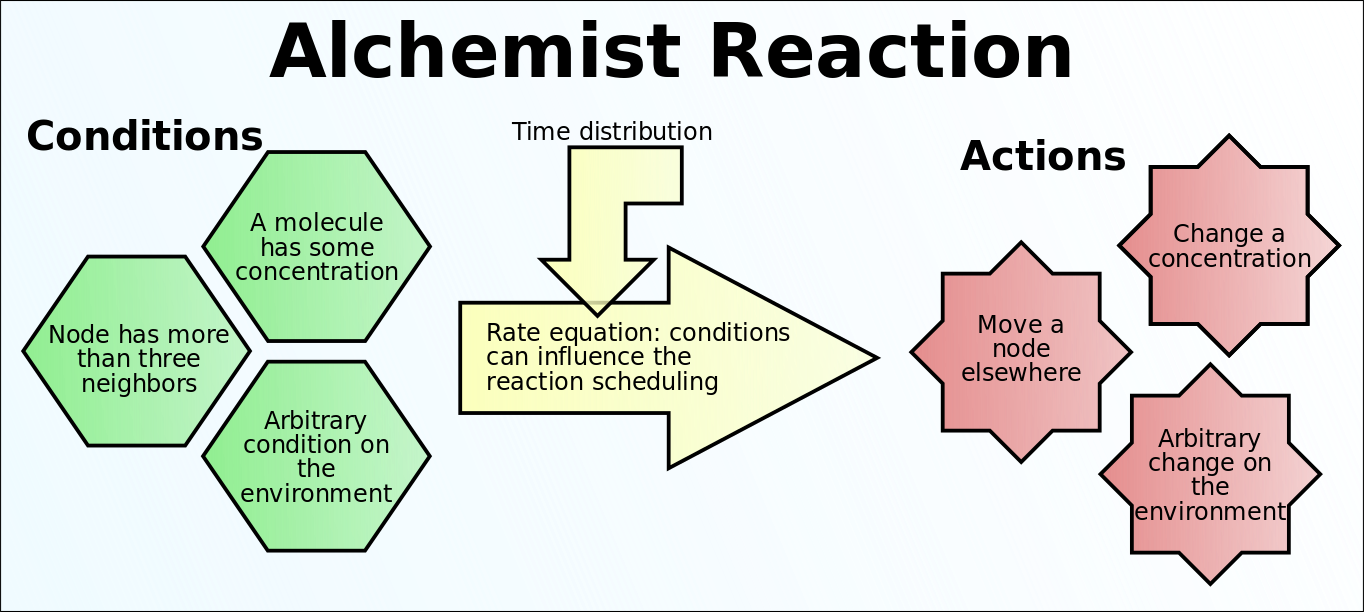
\includegraphics[width=.8\linewidth]{figures/alchemistReaction.png}
    \caption{Rappresentazione di una reazione in Alchemist}\label{fig:reactionAlchemist}
\end{figure}
\begin{figure}[ht]
    \centering
    \includegraphics[width=.8\linewidth]{figures/alchemistModel.png}
    \caption{Il modello di Alchemist}\label{fig:rmodelAlchemist}
\end{figure}
\clearpage

\section{Simulazione di riferimento}\label{refSim}
La simulazione utilizzata come riferimento per questo progetto di tesi è presente nella libreria
di modelli di NetLogo\space\cite{wilensky1997netlogo}. Il modello di riferimento è ``Slime``\space\cite{wilensky1997netlogo}
e per simulare l'aggregazione di tanti singoli organismi in un gruppo si fa riferimento al comportamento delle tartarughe.
Quest'ultime si muovono in uno spazio a griglia e durante il loro movimento rilasciano una particolare molecola
chiamata ``feromone'' che si deposita in una posizione precisa. L'intero mondo è quindi suddiviso
in tantissime ``micro-aree'' chiamate patch. La tartaruga per muoversi 
``annusa'' davanti a se, ovvero percepisce se nelle patch vicine è presente del ``feromone''. Se il valore di quest'ultimo è abbastanza alto, la 
tartaruga si sposterà nella posizione ``annusata'', mentre, in caso contrario la tartaruga si muoverà in modo randomico nello spazio circostante. 
Durante tutto ciò, le patches diffonderanno del ``feromone'' alle varie posizioni vicine e, con il passare del tempo,
il ``feromone'' tende ad evaporare (ovvero sparire) dalla griglia.

\section{Overview su slime-mold}
Nel contesto della presente tesi, sulla base della simulazione di riferimento\ref{refSim} e i comportamenti osservati in essa, si è scelto di indagare un altro 
fenomeno dalle caratteristiche estremamente simili: la muffa mucillaginosa.
In natura, l'aggregazione delle cellule di muffa mucillaginosa (detti anche funghi mucillaginosi o, in inglese, slime-mold) rappresenta
comportamento in cui entità individuali interagiscono tra di loro per formare strutture complesse e funzionali. 
Lo slime-mold è un organismo unicellulare ma, talvolta, può trovarsi anche ad agire come un'entità multicellulare. 
Pur non essendo un fungo è spesso classificato nella stessa categoria per via delle sue caratteristiche affini a quelle di questi organismi.
La particolarità principale della muffa mucillaginosa è che può comportarsi come un organismo unicellulare o multicellulare a seconda delle diverse 
condizioni ambientali in cui si trova.
L'habitat principale di questi organismi è il terreno umido, dove di solito si nutrono di foglie morte o di tronchi di alberi in putrefazione.
Quando trova una fonte di cibo, lo slime-mold si aggrega, formando una massa citoplasmatica detta ``plasmodio'', composta da un grande numero cellule. Inoltre,
questa massa può muoversi, ``navigando'' attraverso il terreno in cerca di cibo.
Infatti, se le risorse alimentari scarseggiano o l'ambiente diventa meno ospitale, lo slime-mold può assumere forme diverse: può formare spore, 
resistenti per sopravvivere in condizioni avverse, oppure aggregarsi insieme ad altri individui simili per formare una struttura multicellulare
che si comporta come un'unica entità, condividendone di conseguenza risorse e compiti.

\chapter{Analisi}
\section{Requisiti} %TODO con Aguzzi
Analizzando il modello presente su NetLogo\cite{wilensky1997netlogo}, possiamo individuare 
le caratteristiche e i requisiti che la simualzione dovrà avere:
\begin{itemize}
    \item Entità ``vive'', che si muovono e depositino il feromone.
    \item Un ambiente che gestisca la presenza del feromone; in particolare dovrà:
    \begin{itemize}
        \item Permettere il depositarsi della sostanza.
        \item Diffondere la sostanza.
        \item Evaporare la sostanza.
    \end{itemize}
    \item Le entità dovranno avere un concetto di direzione.
    \item Il movimento deve seguire delle regole ben precise.
\end{itemize}

\chapter{Design}
\section{Layer}
Si pensi alla simulazione come se fosse un micro-mondo, una ``città'' complessa
e ricca di informazioni. È di interesse capire il livello di temperatura oppure di inquinamento nelle varie aree cittadine, dati invisibili
all'occhio umano ma comunque presenti nell'ambiente e percepibili da chi lo abita. Si ha bisogno
di inserire nell'ambiente degli ``strati'' invisibili che hanno il compito di raccogliere queste informazioni.
È possibile, in Alchemist, definire questi ``strati'' di dati, chiamati Layer.
\newline
Nel contesto di questo progetto è stato necessario l'utilizzo di un Layer che avesse la funzione di ``rete di raccolta''
dei feromoni che, nella simulazione di riferimento\space\ref{refSim}, venivano rilasciati dalle tartarughe nelle varie posizioni
dello spazio. In questo caso il layer ha la stessa dimensione dell'ambiente, in modo tale da poter suddividere l'intera area nelle varie patch di cui si 
è discusso sopra.
Il layer, chiamato \textit{PheromoneLayer} ha come compiti:
\begin{itemize}
    \item Implementare una struttura dati per tenere traccia della quantità di feromone presente in ogni posizione.
    \item Offrire un modo per aggiornare i valori del feromone.
    \item Condividere con le altre classi la struttura dati contenente la quantità di feromone per una specifica posizione.
    \item Lasciare la possibilità all'utente di decidere le dimensioni dell'area totale di riferimento e di ogni patch.
\end{itemize}

\subsection{Le posizioni}
Un aspetto di particolare rilevanza è stato il processo decisionale relativo alla gestione delle posizioni collegate 
al deposito del feromone. Nella simulazione di riferimento\space\ref{refSim} si trova uno spazio a griglia, dove l'area totale è suddivisa
in ``micro-aree'' chiamate patch. In Alchemist, tuttavia, non è presente il concetto di ``area'' o ``spazio'', necessario per individuare una patch,
in quanto le posizioni sono puntiformi e non necessariamente hanno coordinate intere. Il layer sviluppato ricalca l'area (rettangolare o quadrata) del sistema iniziale,
implementando anche un sistema di conversione che trasforma la posizione puntiforme in modo tale da emulare la presenza di una ``area'' bidimensionale, a forma di quadrato, che corrisponde alla patch.
Entrambe le misure, ovvero quella della griglia e quella della patch sono dinamiche e possono essere modificate dall'utente.

\begin{figure}[h!]
    \centering
    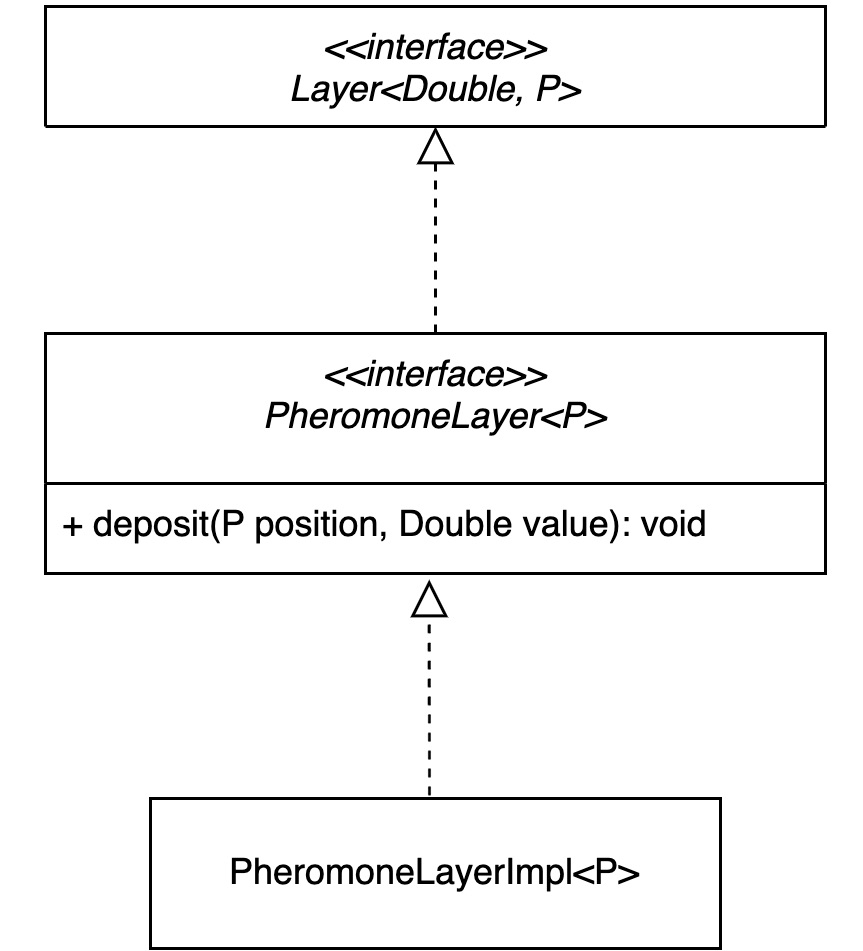
\includegraphics[width=.8\linewidth]{figures/pheromoneLayer.jpeg}
    \caption{Struttura PheromoneLayer}\label{fig:phLayer}
\end{figure}
%You may also put some code snippet (which is NOT float by default), eg: \cref{lst:random-code}.

%\lstinputlisting[float,language=Java,label={lst:random-code}]{listings/HelloWorld.java}

\chapter{Implementazione}

\chapter{Evaluation}
\chapter{Conclusioni e ringraziamenti}
%----------------------------------------------------------------------------------------
% BIBLIOGRAPHY
%----------------------------------------------------------------------------------------

\backmatter\nocite{*} % comment this to only show the referenced entries from the .bib file

\bibliographystyle{alpha}
\bibliography{bibliography}

\end{document}